\documentclass[12pt]{article}
 
\usepackage[margin=1in]{geometry} 
\usepackage{amsmath,amsthm,amssymb}
\usepackage{graphicx}
\usepackage{float}
\usepackage{tikz}
\usetikzlibrary{arrows,shapes,trees} % loads some tikz extensions
 
\begin{document}
 
\title{Homework 5}
\author{Josh Klontz
CSE 802}
 
\maketitle

\begin{enumerate}
\item \subitem{8.}
\begin{enumerate}
\item \textbf{Show that the Bayes rate for the one-dimensional case where $P(w_i)=1/c$ and ... is $P^* = r$.}
\begin{equation}
\begin{split}
p(x) &= c\int p(x|w_i)P(w_i) dx \\
       &= c((\frac{cr}{c-1}) + (1 - \frac{cr}{c-1}))(1/c) \\
       &=1 \\
P^* &= \int min(1-P(w_i|x)) dx \\
      &= \int min(1-p(x|w_i)P(w_i)/p(x)) dx \\
      &= \int min \left(1-\left\{ \begin{array}{rl} 1 & 0\leq x \leq \frac{cr}{c-1} \\ 1 & i \leq x \leq i+1-\frac{cr}{c-1} \\ 0 & \text{elsewhere} \end{array} \right. \cdot 1/c \right) dx \\
      &= \int_0^\frac{cr}{c-1}1-\frac{1}{c}dx~~\text{(The only region where the error rate isn't zero.)} \\
      &= \frac{cr}{c-1}(1-\frac{1}{c}) \\
      &= \frac{cr}{c-1} - \frac{r}{c-1} \\
      &= \frac{cr-r}{c-1} \\
      &= r\frac{c-1}{c-1} \\
      &= r \\
      & \qed
\end{split}
\end{equation}
\item \textbf{Show that for this case the nearest-neighbor rate is $P=P^*$}
\begin{equation}
\begin{split}
P &= \int \left[1-\sum_{i=1}^c P^2(w_i|x) \right]p(x)dx \\
   &= \int \left[1-\sum_{i=1}^c (p(x|w_i)P(w_i)/p(x))^2 \right]p(x)dx \\
   &= \int 1-c \left( \left\{ \begin{array}{rl} 1/c^2 & 0\leq x \leq \frac{cr}{c-1} \\ 1/c^2 & i \leq x \leq i+1-\frac{cr}{c-1} \\ 0 & \text{elsewhere} \end{array} \right. \right)^2 dx \\
   &= \int 1- \left\{ \begin{array}{rl} 1/c & 0\leq x \leq \frac{cr}{c-1} \\ 1/c & i \leq x \leq i+1-\frac{cr}{c-1} \\ 0 & \text{elsewhere} \end{array} \right. dx \\
   &= \int_0^\frac{cr}{c-1}1-1/c~dx~~\text{As $n \to \infty$ this is the only term with non-zero error.} \\
   &= ...~\text{Same algebraic simplificaiton as (a)} \\
   &=r \\
   &=P^* \\
   & \qed
\end{split}
\end{equation}
\end{enumerate}
\subitem{9.}
\begin{equation}
\begin{split}
m_1 &= [5 -4] \\
m_2 &= [3.33 6.67] \\
m_3 &= [2.33 2] \\
\end{split}
\end{equation}
\newpage
\begin{enumerate}
\item \textbf{Plot the decision boundary for $w_1$ and $w_2$.}
\begin{figure}[H]
\centering
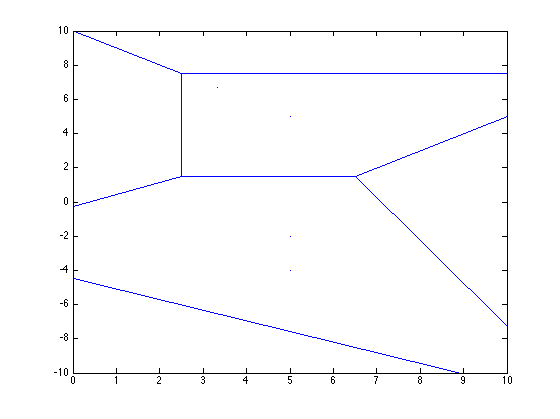
\includegraphics[width=5in]{12.png}
\end{figure}
\item \textbf{Plot the decision boundary for $w_1$ and $w_3$.}
\begin{figure}[H]
\centering
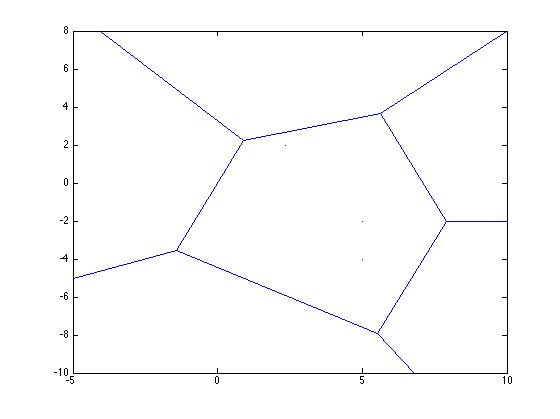
\includegraphics[width=5in]{13.png}
\end{figure}
\newpage
\item \textbf{Plot the decision boundary for $w_2$ and $w_3$.}
\begin{figure}[H]
\centering
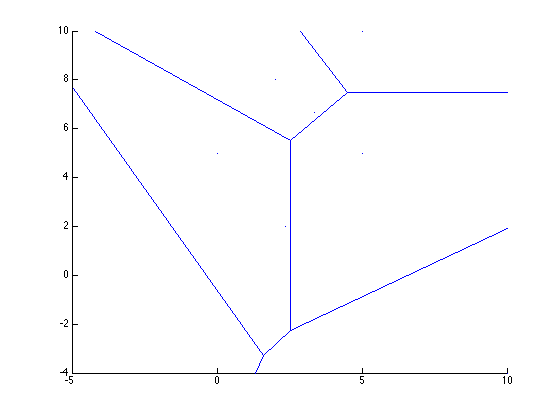
\includegraphics[width=5in]{23.png}
\end{figure}
\item \textbf{Plot the decision boundary for $w_1$, $w_2$, and $w_3$.}
\begin{figure}[H]
\centering
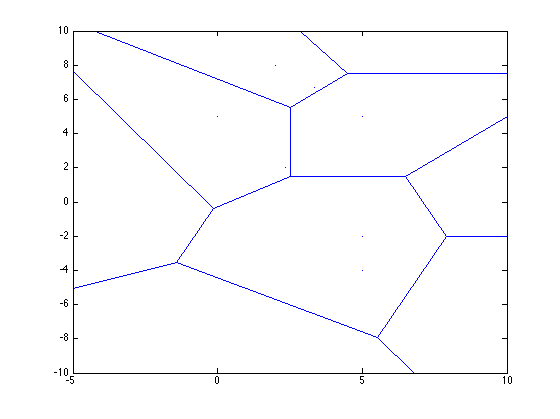
\includegraphics[width=5in]{123.png}
\end{figure}
\end{enumerate}
\newpage
\subitem{19.} \textbf{Consider the Euclidean metric in $d$ dimensions ...}

A space is a metric space if for all vectors $a$, $b$, and $c$:
\begin{equation}
\begin{split}
D(a,b) &\geq 0 \\
D(a,b) &= 0 \iff a=b \\
D(a,b) &= D(b,a) \\
D(a,b) &+ D(b,c) \geq D(a,c) \\
\end{split}
\end{equation}
We will prove that the Euclidean distance metric with scaled axes is a metric space by proving each of the four properties individually.
\begin{equation}
D(a,b) = \sqrt{\sum_{k=1}^d(\alpha_k x_k-\alpha_k y_k)^2}
\end{equation}
\begin{enumerate}
\item Nonnegativity: $ D(x,y) \geq 0 $ \\
From the problem definition it is assumed that $\alpha$, $x$, and $y$ are real-valued vectors. Therefore, $\alpha_k x_k-\alpha_k y_k$ is a real value for all $k$. Thus the quantity $(\alpha_k x_k-\alpha_k y_k)^2$ is greater than or equal to 0. It follows that the sum of these quantities and the square root of said sum are also greater than or equal to 0.
\item Reflexivitiy: $ D(x,y) = 0 \iff a=b $
\begin{itemize}
\item $a = b \implies D(x,y) = 0$ \\
If $a = b$ then the quantity $\alpha_k x_k-\alpha_k y_k$ is zero for all $k$. It follows that the quared sum of these quantities and the square root of said sum are also equal to 0.
\item $a \neq b \implies D(x,y) \neq 0$ \\
If $a \neq b$ then there exists a quantity $\alpha_k x_k-\alpha_k y_k$ that is not zero for some $k$. From the nonnegativity property already proven, it follows that the square of this term is positive and therefore the squared sum is positive and thus not equal to 0.
\end{itemize}
\item Symmetry: $ D(x,y) = D(y,x) $ \\
Note that each term $(\alpha_k x_k-\alpha_k y_k)^2$ is symmetric because swapping the variables $x_k$ and $y_k$ changes the sign of the subtraction but not the value after it is squared. It follows that the sum of these values and the square root of said sum are also symmetric.
\item Triangle Inequality: $ D(x,y) + D(y,z) \geq D(x,z) $ \\
Let $g_{xy} = \alpha_k x_k-\alpha_k y_k$ in $\sqrt{\sum_{k=1}^dg_{xy}^2} + \sqrt{\sum_{k=1}^dg_{yz}^2} \geq \sqrt{\sum_{k=1}^dg_{xz}^2}$. From the problem statement we know that $g$ is a real valued vector and. From the non-negativity property it follows that $\sum_{k=1}^dg_{xy}^2 + \sum_{k=1}^dg_{yz}^2 \geq \sum_{k=1}^dg_{xz}^2$. Note that this is Cauchy–Schwarz inequality for vectors in an inner product space.\\
\qed
\end{enumerate}
\newpage
\item Fisher Iris
\begin{enumerate}
\item PCA
\begin{figure}[H]
\begin{verbatim}
d = csvread('iris.txt')
l = d(:,5)
f = d(:,[1 2 3 4])
m = mean(f)
cf = f - repmat(m, 150, 1)
s = transpose(cf)*cf
[v, d] = eig(s)
fp = cf * v(:,[3 4])
plot(fp(:,1), fp(:,2), '.')
\end{verbatim}
\caption{MATLAB code to compute and plot subspace.}
\end{figure}
\begin{figure}[H]
\centering
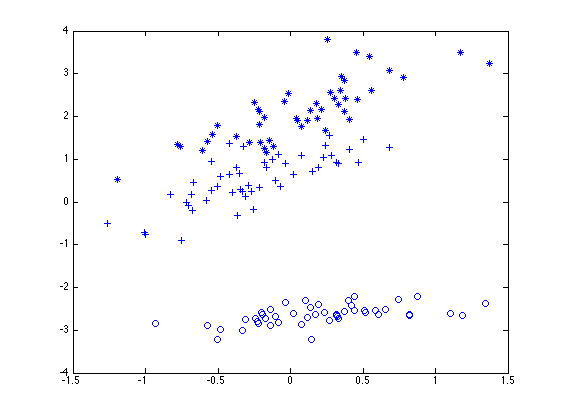
\includegraphics[width=5in]{2a}
\caption{First two eigenvalues.}
\end{figure}
Retained variance = 97.76\%
\item Bayesian classifier \\
\begin{figure}[H]
\begin{verbatim}
function [error_rate] = bayesian_classifier(training, testing)
    training_data = training(:, 1:size(training,2)-1);
    training_labels = training(:, size(training,2));
    testing_data = training(:, 1:size(testing,2)-1);
    testing_labels = training(:, size(testing,2));
    unique_labels = unique(training_labels);
    class_means = {};
    class_covariances = {};
    for label = 1:size(unique_labels,1)
        class_data = training_data(training_labels==label,:);
        class_means{label} = mean(class_data);
        class_covariances{label} = cov(class_data);
    end
    errors = 0;
    for index = 1:size(testing_data,1)
        highest_pdf = 0;
        highest_label = -1;
        for label = 1:size(unique_labels,1)
            pdf = mvnpdf(testing_data(index,:),...
                         class_means{label},...
                         class_covariances{label});
            if pdf > highest_pdf
                highest_pdf = pdf;
                highest_label = label;
            end
        end
        if (highest_label ~= testing_labels(index,:))
            errors = errors + 1;
        end
    end
    error_rate = errors / size(testing_data,1);    
end
error = crossval(@bayesian_classifier, fpl, 'kfold', 5)
\end{verbatim}
\caption{MATLAB code for Bayesian classifier.}
\end{figure}
\newpage
\item Parzen window classifier
\begin{figure}[H]
\begin{verbatim}
function [error_rate] = parzen_window_classifier(training, testing)
    h = 0.5; % Change window size here
    training_data = training(:, 1:size(training,2)-1);
    training_labels = training(:, size(training,2));
    testing_data = training(:, 1:size(testing,2)-1);
    testing_labels = training(:, size(testing,2));
    unique_labels = unique(training_labels);
    errors = 0;
    for index = 1:size(testing_data,1)
        densities = [0 0 0];
        for training_index = 1:size(training_data,1)
            training_label = training_labels(training_index,1);
            delta = training_data(training_index,:)-...
                    testing_data(index,:);
            densities(training_label) = densities(training_label) + ...
                                        normpdf(delta*transpose(delta)/h);
        end
        highest_weight = 0;
        highest_label = -1;
        for label = 1:size(unique_labels,1)
            if densities(label) > highest_weight
                highest_weight = densities(label);
                highest_label = label;
            end
        end
        if (highest_label ~= testing_labels(index,:))
            errors = errors + 1;
        end
    end
    error_rate = errors / size(testing_data,1);    
end
\end{verbatim}
\caption{MATLAB code for Parzen window classifier.}
\end{figure}
\newpage
\item 1-NN classifier
\begin{figure}[H]
\begin{verbatim}
function [error_rate] = nn_classifier(training, testing)
    training_data = training(:, 1:size(training,2)-1);
    training_labels = training(:, size(training,2));
    testing_data = training(:, 1:size(testing,2)-1);
    testing_labels = training(:, size(testing,2));
    errors = 0;
    for index = 1:size(testing_data,1)
        closest_distance = realmax();
        closest_label = -1;
        for training_index = 1:size(training_data,1)
            delta = training_data(training_index,:)-...
                    testing_data(index,:);
            distance = delta*transpose(delta);
            if distance < closest_distance
                closest_distance = distance;
                closest_label = training_labels(training_index,1);
            end
        end
        if (closest_label ~= testing_labels(index,:))
            errors = errors + 1;
        end
    end
    error_rate = errors / size(testing_data,1);    
end
\end{verbatim}
\caption{MATLAB code for 1-NN classifier.}
\end{figure}
\item Error Rates
\begin{table}[H]
\begin{tabular}{ccc}
Classifier & Average Error & Error Standard Deviation \\ \hline
Bayesian & 0.03 & 0.01 \\
Parzen Window (h=0.01) & 0 & 0 \\
Parzen Window (h=0.5) & 0.048 & 0.007 \\
Parzen Window (h=10) & 0.22 & 0.04 \\
1-NN & 0 & 0 \\
\end{tabular}
\caption{Error rates for each classifier.}
\end{table}
\end{enumerate}
\end{enumerate}
\end{document}
